\section{Preliminaries}
\label{sec:pois_review}
\subsection{Poisson Surface Reconstruction}
We denote the indicator function of a model $M$ as $$ \chi_M(\vect{x}) :=
\begin{cases}
1, & \text{if }\vect{x}\text{ is in the interior of the model } M \\
\frac{1}{2}, & \text{if } \vect{x}\text{ is on the model's surface}\\
0, & \text{if }\vect{x}\text{ is exterior to } M
\end{cases}. $$
The key observation of the Poisson surface reconstruction formulation, is that if one obtains a function $\vec{V}(\vect{x})$ with $\vec{V}(\vect{x})\approx{\nabla}\chi_M$, that approximates the smoothed gradient of the indicator function, finding an approximation to the indicator function reduces to finding a $\inda$ such that {\small 
\begin{equation} \label{eq:poisson}
	\lapl{\inda} = {\grad} \cdot \vec{V}.
\end{equation}}
We define the set of input surface points to be $P:=\{(\vect{p}_1,\vect{n}_1), (\vect{p}_2,\vect{n}_2) \hdots (\vect{p}_M,\vect{n}_M) : (\vect{p}_i,\vect{n}_i) \in \realn^3 \times \realn^3 \}$ where $\vect{p}_i$ and $\mathbf{n}_i$ are the position and normal vector of the $i^{th}$ sample respectively. Orientation can be succinctly represented with only two values, however, it is convenient to keep it as the normal at a point, because the length of the normal can be used to encode the sampling density of the point-set at a point. For the following discussion, we also need to introduce the notation $\patch_{\vect{s}}$, which denotes a patch of the surface model about the sample location $\vect{s}$. 

Inspired by the approach of Kazhdan et al.~\cite{Kazhdan06} the approximation $\vec{V}(\vx)$ is defined to be  {\small 
\begin{eqnarray}
	\vec{V}(\vx) & := & \sum_{(\vect{s},\vect{n}) \in P}\left|\patch_s\right|F(\vx-\vect{s})\cdot\vn \label{eq:vdef} \\
	 & \approx & \sum_{(\vect{s},\vect{n}) \in P} \int_{\patch_s}{F(\vect{x} - \vect{p}) \nabla \chi (\vect{p})} \mathrm{d} \vect{p}. \notag  
\end{eqnarray}}
Thus, $\vec{V}(\vx)$ approximates the gradient of the indicator smoothed by some filter $F$, broken up over surface patches of the model. We assume the point sampling to be uniform, thus the area of each patch $\left|\patch_s\right|$ should be a constant, and our resulting approximation will be scaled by an unknown factor. We return to this in \SC{sec:levelset}. The choice of $F$ places computational constraints on the resulting algorithm.

$F$ is often explicitly chosen to be a compactly supported function. This simplifies and reduces the computational cost of the method when used in conjunction with an oct-tree based representation of $\vec{V}(\vx)$ \cite{Kazhdan06}. However, the  disadvantage of this choice is that $F$ may over smooth data in areas of high curvature \cite{reconbench}, much in the same way that a representation of a sampled signal may fail to take advantage of the full approximation power of the function space in which it is represented if it is not properly prefiltered. Theoretically, one could simply reconstruct the surface at higher resolutions, allowing the basis functions to become more ``fine'', but increasing the total amount of memory used. On a regular grid, this is undesirable. Another approach is to impose a type of ``interpolation'' constraint on the original data \cite{screenedk} (\SC{sec:vari_review}).

Ideally, the filter $F$ should correspond to some globally supported RBF. However, as the support of $F$ grows, so does the cost of evaluating it at lattice sites. Moreover, the added benefit of a globally supported RBF is partially lost as the subsequent steps are entirely lattice-based and do not take the RBF into consideration. Our approach circumvents the choice of $F$ entirely by posing the gradient approximation problem as a variational problem that, in addition to imposing the interpolation constraint, also imposes constraints on the ``compactness'' and ``smoothness'' of the gradient approximation. The only kernel we need to consider is the one that generates our target shift-invariant space, i.e. the space used to recover the smoothed indicator function. This type of variational reconstruction can be seen as an approximation to radial basis approaches~\cite{variational}, and is well-suited to our Poisson formulation in shift-invariant spaces.

Before presenting our approach (\SC{sec:pipeline}), we review the necessary background behind shift-invariant spaces and its connection to irregular sampling.

\subsection{Sampling Lattices} \label{sec:smpl_review}
In the univariate case, there is only one way to uniformly sample a signal: take equally spaced samples along the independent axis. However, when sampling multivariate signals the situation is not as straightforward. A common approach is to inherit the ideas from the univariate case and sample the function at regular intervals in each axis -- a Cartesian sampling --  while another might be to place samples at the centres of spheres arranged in the densest possible sphere packing (otherwise known as an FCC sampling). If $\mathbf{L}$ is a unimodular matrix, the set $\lattice{L} := \{\mathbf{L}\cdot\vect{n} : \vect{n} \in \intn^3 \}$ represents all possible sampling lattices. $\mathbf{L}$ is often called the \emph{generating matrix} for a lattice, and we'll assume that $\mathbf{L}$ is normalized so that $\left|\det\mathbf{L}\right| = 1$. The lattice's dual, denoted by $\duallattice{L}$, is the lattice generated by $\mathbf{L}^{-T}$. Finally, to control the sampling rate of a function a uniform scaling parameter $h$ is introduced -- lattices scaled by this parameter will be denoted by $\lattice{L}_h$. Typically, for the problem of surface reconstruction, our input data are not uniformly distributed in space, or even about the surface of the model, but the concept of a sampling lattice is fundamental in forming the definition of our target approximation spaces (\SC{sec:sis_review}).

The Cartesian lattice is given by the generating matrix $\mathbf{L}_C:=\mathbf{I}_3$, where $\mathbf{I}_3$ is the $3 \times 3$ identity matrix. There are many factors that contribute to the ubiquity of the Cartesian lattice in practice. Possibly one of its most attractive features is its separability. Owing to this, the implementation of generating functions that span function spaces on the Cartesian lattice may be realized by a tensor product extension of existing univariate techniques. Filtering techniques are also easy to implement, as the Fast Fourier Transform is  separable and may be applied independently to each axis of the data. However, in terms of sampling efficiency, the BCC lattice is the optimal lattice in $\realn^3$, while the Cartesian is sub-optimal.

The Body-Centered Cubic (BCC) lattice is generated by the matrix  {\footnotesize
\begin{equation*} 
	\mathbf{L}_B := \frac{1}{\sqrt[3]{4}}
	\begin{bmatrix}
		-1 & 1 & 1 \\ 
		1 & -1 & 1 \\ 
		1 & 1 & -1 
	\end{bmatrix}.
\end{equation*}}
However, the BCC lattice is non-separable, and requires special care in data retrieval and indexing. \FG{fig:lattices} shows these lattices and their Voronoi regions, including the dual of the BCC lattice, the FCC lattice (the Cartesian lattice is dual to itself.)

\subsection{Shift Invariant Spaces} \label{sec:sis_review}
As our target reconstruction spaces, we consider the shift-invariant spaces defined by {\small 
\begin{equation*}
	\fspce{\varphi}{ \lattice{L}_h} := \left\{ g(\vx) := \displaystyle\sum_{\vect{m} \in \intn^3} c[\vect{m}]\genfuncdef{\vx} : c \in \ell_2 \right\},
\end{equation*}}
where $\varphi$ is the generating function for the space, $h$ is a scaling parameter that controls the sampling rate or granularity, and $\mathbf{L}$ is the generating matrix for a given sampling lattice. Representing a function $f$ in a shift invariant space boils down to finding an appropriate coefficient $c[\vect{m}]$ vector that brings $g$ as close as possible to the true underlying function $f$. 

Typically, as memory is a limited quantity, we are only interested in a finite number of points on a lattice. We denote the set of such points as $\{\vect{s}_1,\vect{s}_2,\ \hdots  \ \vect{s}_N\} \subset \mathbf{L}\intn^3.$ Corresponding to each lattice site is a coefficient $c_k$; we collect all such coefficients in the column vector $\mathbf{c}:=\left[c_1 \ c_2 \ \hdots \ c_N \right]^T.$ We also use the short hand notation $\varphi_k(\vx) := \varphi(\frac{\vx}{h}-\vect{s}_k)$; from this perspective, our function space is now {\small 
\begin{equation}
	\left\{ \displaystyle\sum_{k=0}^N c_k \varphi_k(\vx) \right\} \subset \fspce{\varphi}{\lattice{L}_h}.
\end{equation}}
Further, we denote $\mathbf{\Phii}$ to be the $M \times N$ matrix whose elements are given by sampling the basis functions anchored at each lattice site, or $P_{i,j} := \varphi_j(\vx_i)$. Clearly, if our data are sampled at the lattice sites ($\vx_i = \vect{s}_i$), then the problem of finding an interpolative scheme reduces to finding $\vect{c}$ such that $\mathbf{\Phii c=f},$ which only involves inverting the square matrix $\mathbf{\Phii}.$ However, our sample locations are almost certain to not coincide with lattice sites and we must consider alternative schemes for finding $\mathbf{c}$, which we'll come back to in \SC{sec:vari_review}

\subsection{Error Analysis} \label{sec:sis_error}
To facilitate the classical analysis of signals in a shift-invariant space, we need a few notions first. We define all this notation in $s$-dimensions, as the generalization comes at little cost. The first tool we need is the Fourier transform of a multivariate function $f(\vect{x})$, which we define as $ \ft{f}(\vect{\omega}) := \int_{\reel^s} f(\vect{x}) \exp(-2\pi \imath \vect{\omega} \cdot \vect{x}) \mathrm{d}\vect{x} $. The discrete time Fourier transform (DTFT) of a sequence $c[\cdot]$ associated with a lattice $\lattice{L}$ is defined as $\ft{C}(\vect{\omega}) := \sum_{\vect{m}  \in \ints^s} c[\vect{m}] \exp(-2 \pi \imath \vect{\omega} \cdot (\mat{L}\vect{n}))$. Recall that $\ft{C}(\vect{\omega})$ is periodic with respect to the dual lattice $\duallattice{L}$, i.e. $\ft{C}(\vect{\omega} + \invtransp{\mat{L}} \vect{m}) = \ft{C}(\vect{\omega}), \forall \vect{m} \in \ints^s$. The notation `$\ftpairs{}{}$' is subsequently employed to denote transform pairs, i.e. $\ftpairs{f(\vect{x})}{\ft{f}(\vect{\omega})}$ (Fourier transform pairs) and $\ftpairs{c[\vect{m}]}{\ft{C}(\vect{\omega})}$ (DTFT pairs).

The closed unit hypercube $[0,1]^s$ is denoted as $\ucube^s$ while the closed hypercube $[-1,1]^s$ is denoted as $\cube^s$. The corresponding open hypercubes are denoted as $\oucube^s$ and $\ocube^s$ respectively. The inner product between two real valued functions $f_1$ and $f_2$ belonging to $L_2(\reel^s)$ is denoted as $\ip{f}{g} := \int_{\reel^s} f(\vect{x}) g(\vect{x}) d\vect{x}$. Likewise, the inner product between two functions $f_1$ and $f_2$ that belong to $L_2(\cube^s)$ is denoted as $\innerproduct{f_1}{f_2} := {2^{-s}} \int_{\cube^s} f_1(\vect{x}) f_2(\vect{x}) d\vect{x}$. The norms induced by these inner products are denoted as $\Ltwonorm{\cdot}$ and $\LLnorm{\cdot}$ respectively.

In order to ensure that any function $g \in \aspace{\lattice{L}_h}{\varphi}$ has a unique representation in terms of a finite energy coefficient sequence $c[\cdot]$, the lattice translates $\{\varphi(\cdot - \mat{L}\vect{n})\}_{\vect{n}  \in \ints^s}$ must form a Riesz basis~\cite{kreyszig89}, i.e. there exist positive constants $a$ and $b$ such that $\forall c[\cdot] \in l_2(\ints^s)$,
\begin{equation*}
  a \norm{c}^2_{l_2(\ints^s)} \le \Ltwonormbig{\sum_{\vect{n} \in \ints^s}
  c[\vect{n}] \varphi(\vect{x} - \mat{L}\vect{n})}^2 \le b
	\norm{c}^2_{l_2(\ints^s)}.
\end{equation*}


\subsection{The Error Kernel}
The error $\Ltwonorm{f - \appf{f}}$ between $f$ and its approximation
$\appf{f} \in \aspace{\lattice{L}_h}{\varphi}$ can conveniently be
quantified via an error kernel in the Fourier domain. It is defined as
\begin{equation}
	E(\vect{\omega}) := \underbrace{1 - \frac{\abs{\ft{\varphi}(\vect{\omega})}^2}{\ft{A}_{\varphi}(\vect{\omega})}}_{E_{\mathsf{min}}(\vect{\omega})}
	+ 
	\underbrace{
	\ft{A}_{\varphi}(\vect{\omega})
	\abs{\ft{\analysis{\varphi}}(\vect{\omega}) -
 		\ft{\dual{\varphi}}(\vect{\omega})}^2
  	}_{E_{\mathsf{res}}(\vect{\omega})}.
  \label{eq:scErrorKernel}
\end{equation}
For a bandlimited function $f$ whose spectrum is entirely contained
within the Voronoi cell of $\duallattice{L}_h$ centered around $\vect{\omega} = 0$, we have 
\begin{equation}
	\Ltwonorm{f - \appf{f}} = \int_{\reel^s}
	\abs{\ft{f}(\vect{\omega})}^2 E(h\vect{\omega}) d\vect{\omega},
	\label{eq:avgError}
\end{equation}
whereas when $f \in W_2^k(\reel^s)$ with $k > \frac{1}{2}$, the integral in~\eqref{eq:avgError} gives the $L_2$-error averaged over all possible shifts of $f$. Even though this kernel was initially proposed in the univariate setting by Blu and Unser~\cite{blu99}, multivariate non-Cartesian extensions have also appeared in the literature~\cite{condat05hexagonal, condat07, condat08, alim10, condat11}. Note that the minimum-error approximation scenario occurs when $f$ is orthogonally projected to $\aspace{\lattice{L}_h}{\varphi}$, or in other words $\analysis{\varphi}$ is chosen to be $\dual{\varphi}$.
 
\subsection{Approximation Error}

If the generating function that spans the space satisfies the \emph{Strang-Fix} conditions of order $k$, and $f$ belongs to the Sobolev space of at least order $k$, then it can be shown that the minimum approximation error (in the least-squares sense) decays asymptotically as $O(h^k)$, and the space is said to have approximation order $k$. We often only have access to $f$ through a discrete amount of samples, $\mathbf{f} := \left[ f_1 \ f_2 \ \hdots \ f_M \right]^T$ located at sample points $S := \{\vx_1, \vx_2 \hdots \vx_M \}$ respectively. When this is the case, the minimum-error approximation is unattainable. However, interpolative and quasi-interpolative methods \cite{quasibcc,interprev}, which can be seen as oblique projections onto $\aspace{\lattice{L}_h}{\varphi}$, maintain the same order of accuracy.


For sufficiently smooth functions $f$ that are uniformly sampled and properly prefiltered, the trilinear and linear reconstruction filters (Cartesian and BCC respectively) assure second order convergence, while the tricubic and Quintic assure fourth order. Another nicety of these spaces is that data processing techniques --- derivative approximation for example --- can often be represented by a convolution of the coefficient vector with either an \emph{Infinite Impulse Response} (IIR) or \emph{Finite Impulse Response} (FIR) filter. 



\subsection{Box Splines} \label{sec:box_review}
Box splines are compact piece-wise polynomial functions $ M_\mathbf{\Xii} : \realn^s \to \realn.$ The matrix $\mathbf{\Xii}$ denotes a collection of direction vectors, $\mathbf{\Xii} := \left[ \xi_1 \ \xi_2 \hdots \xi_n\right].$ When $n=s$, the function $M_\mathbf{\Xii}(\vx)$ is defined to be ${1}/|{\det\mathbf{\Xii}}|$ inside the polytope formed by the Minkowski sum of the direction vectors of $\mathbf{\Xii}$, and zero otherwise (that is, ${1}/{|\det\mathbf{\Xii}|}$ when $\vx \in \{ \mathbf{\xi}_1 t_1 + \hdots + \mathbf{\xi}_s t_s  : t_i\in [0,1) \})$. When $n > s$, the box spline is recursively defined as {\small 
\begin{equation} \label{eq:box_def}
	M_{\mathbf{\Xii}}(\vx) := \int_0^1{\!M_{\mathbf{\Xii/\xi}_n}(\vx - t\mathbf{\xi}_n)} \mathrm{d}t,
\end{equation}}
where ${\mathbf{\Xii/\xi}_n}$ is the matrix obtained by removing the column vector $\xi_n$ from $\mathbf{\Xii}$. Box splines are a natural fit for our purposes, and are chosen to span our function spaces. One motivating factor that encourages the use of box splines on the BCC lattice over the Cartesian lattice is that the support of the box splines on the BCC lattice contains less lattice sites as opposed to their Cartesian counterparts. At the same time, they maintain the same order of accuracy and smoothness. This implies that one should expect roughly the same quality reconstruction, with less memory accesses per reconstructed value.

The evaluation of a box spline, in general, can be achieved by evaluating a simple recursive expression \cite{boorboxsplines}. However, for many purposes, this form of evaluation is too slow. There has been a line of research \cite{firstbox} aimed towards obtaining fast piecewise polynomial representations of the box splines on the BCC lattice, and showing their advantage in speed and accuracy over splines on the Cartesian lattice when the data to be interpolated are sufficiently smooth.

\begin{figure}
  \centering
  \mbox{} \hfill
	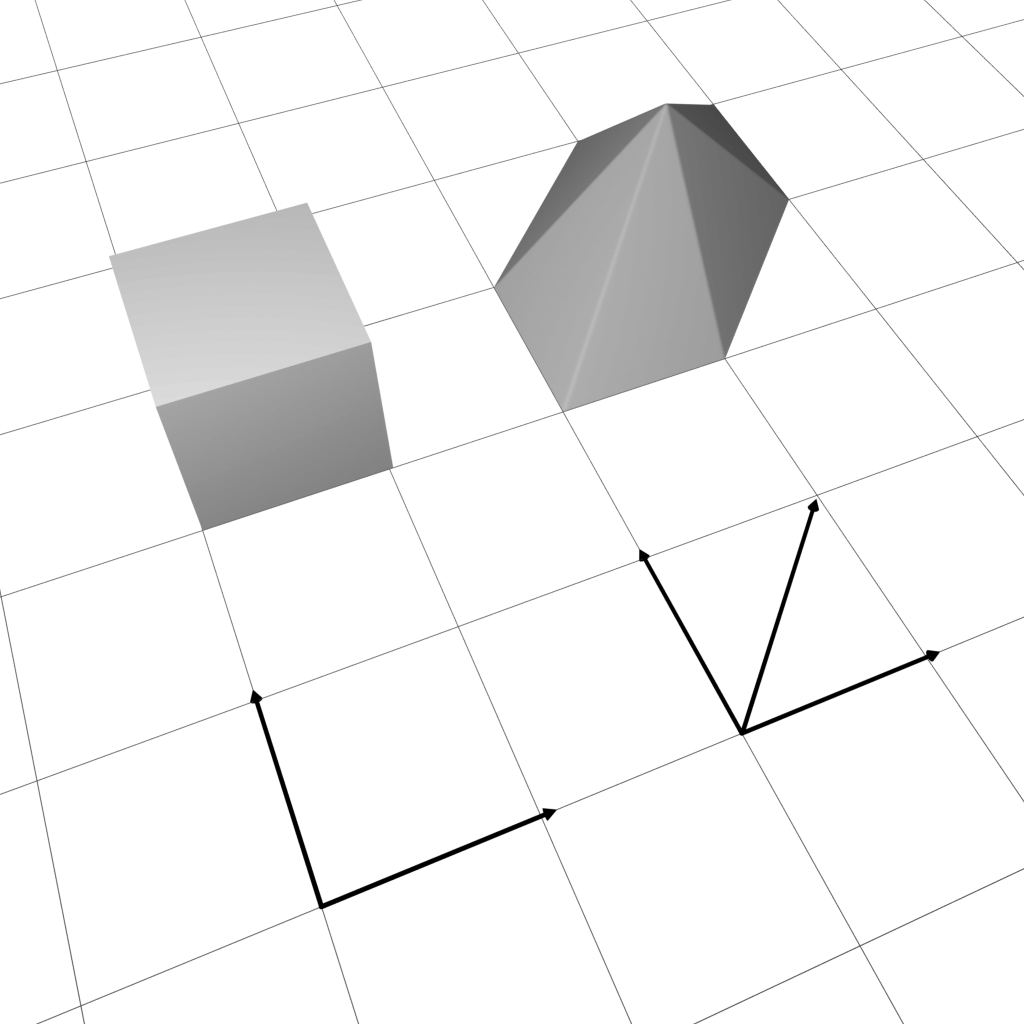
\includegraphics[width=\linewidth]{figures/boxspline/2dex}
  \caption{\label{fig:box2d}%
  An example of box splines in 2D. On the left is the box spline comprised of the direction vectors $\mathbf{\xi}_1, \mathbf{\xi}_2$, (the case n=s) which is the indicator function of the Minkowski sum of the vectors. The box spline on the right, includes a third vector $\mathbf{\xi}_3$, which can be thought of as ``smearing'' the first spline along the direction $\mathbf{\xi}_3$.
  }
\end{figure}


\subsection{Irregular Sampling}
\label{sec:vari_review}
%When reconstructing functions whose data are sampled regularly on a lattice, finding an oblique projection of the original function in the target function space is relatively straight-forward. However, except on very rare occasions, samples placed over the surface of a model do not coincide with lattice sites. A solution to this problem is to ``re-sample'' the input point set onto said lattices sites.
In the work by Kazdhan et al. \cite{fftk} the range data, $P$, are splatted via a linear filter onto a regular Cartesian grid. This tends to over-smooth the resulting reconstruction, as it allows the surface to deviate from the original sample locations. Ideally, we would like to find a function that not only interpolates the input data, but provides the representation with the smallest possible ``shell'' about the initial point set (i.e., the fewest non zero coefficients) while still interpolating the data and eliciting a unique solution. 

Thus, we recast the problem of finding a representation of $g$ within our function space as an optimization problem. There are similar works that impose variational constraints on random point samples for images \cite{variational}, as well as multi-resolution techniques for volumetric data \cite{onvari} and an extension to box spline spaces \cite{xu2012rec}. In the same vein, we seek a function $g \in \aspace{\lattice{L}_h}{\varphi}$ that attempts to interpolate the input data, and minimize a functional $E$. Specifically, we seek a $g$ that minimizes {\small 
\begin{equation} \label{eq:minexp}
 	\sump_{i=1}^{M} (g(\vx_i) -  f_i)^2 + E(g).
\end{equation}}
It is important to introduce a bit of notation before proceeding, $\dv{\mathbf{v}} f := \mathbf{v} \cdot \grad f$ defines the directional derivative of $f$ in the direction $\mathbf{v}$. The Beppo-Levi inner product of order $n$ is defined as $\blip{n}{f}{g}:= \sum_{|\mathbf{p}|=n}({n!}/{\mathbf{p}!}) \innerp{\mathbf{D^p}f}{\mathbf{D^p}g}$, where $\mathbf{p}$ is an integer vector such that $\left| \mathbf{p}\right| := p_1 + p_2 + p_3 $. We also use the short hand $\mathbf{D^p}f := \partial^{\left| \mathbf{p}\right|}f/({\partial^{p_1}x_1}{\partial^{p_2}x_2}{\partial^{p_3}x_3}).$ The second order Beppo-Levi norm of $f$ is defined as $\bln{2}{f}^2:=\blip{2}{f}{f}$.

The second order Beppo-Levi norm can be thought to measure the ``smoothness'' of a function. However, constraining the smoothness of our approximation alone is not sufficient to elicit the desired solution in our case. We propose that the smoothed normal field should also minimize the inner product of the function with itself. This has the physical interpretation of forcing the solution to be close to zero everywhere except near the input points. Our proposed cost functional is then $E(g) := \lambda_1 \left|\left|{g}\right|\right| + \lambda_2 \bln{2}{g}.$ Here, $\lambda_1$ controls the amount to which the function is penalized for large coefficient values. When combined with the interpolation constraint, this imposes the behavior of forcing the function to be zero away from the surface. The parameter $\lambda_2$ controls the smoothness of the resulting normal field.
%\begin{equation} \label{eq:functional}
%	E(g) := \lambda_1 \left|\left|{g}\right|\right| + \lambda_2 \bln{2}{g}.
%\end{equation}

Finding $g$ that minimizes equation \EQ{eq:minexp} involves rewriting the minimization problem in terms of $\mathbf{c}$ \cite{xu2012rec}. Following some straightforward algebraic manipulations (see \cite{xu2012rec} for details), the coefficient vector can be obtained by taking $\mathbf{c} = ( \mathbf{\Phii}^T\mathbf{\Phii} + \lambda_1\mathbf{G} + \lambda_2\mathbf{S})^{-1}\mathbf{\Phii}^T\mathbf{f}$, where $G_{i,j}:=\innerp{\varphi_i}{\varphi_j}$, $S_{i,j}:=\blip{2}{\varphi_i}{\varphi_j}$, and $P_{i,j} := \varphi_j(\vx_i)$ as before. Since $\varphi$ is known in closed form in our test cases, the entries of both $\mathbf{G}$ and $\mathbf{S}$ can be evaluated analytically. The above vector equation can be solved using the Conjugate Gradient method.
